\documentclass[]{article}
\usepackage{lmodern}
\usepackage{amssymb,amsmath}
\usepackage{ifxetex,ifluatex}
\usepackage{fixltx2e} % provides \textsubscript
\ifnum 0\ifxetex 1\fi\ifluatex 1\fi=0 % if pdftex
  \usepackage[T1]{fontenc}
  \usepackage[utf8]{inputenc}
\else % if luatex or xelatex
  \ifxetex
    \usepackage{mathspec}
  \else
    \usepackage{fontspec}
  \fi
  \defaultfontfeatures{Ligatures=TeX,Scale=MatchLowercase}
\fi
% use upquote if available, for straight quotes in verbatim environments
\IfFileExists{upquote.sty}{\usepackage{upquote}}{}
% use microtype if available
\IfFileExists{microtype.sty}{%
\usepackage{microtype}
\UseMicrotypeSet[protrusion]{basicmath} % disable protrusion for tt fonts
}{}
\usepackage[margin=1in]{geometry}
\usepackage{hyperref}
\hypersetup{unicode=true,
            pdftitle={Patagonia parrots density analysis},
            pdfauthor={Francisco Dénes and Peter Sólymos},
            pdfborder={0 0 0},
            breaklinks=true}
\urlstyle{same}  % don't use monospace font for urls
\usepackage{color}
\usepackage{fancyvrb}
\newcommand{\VerbBar}{|}
\newcommand{\VERB}{\Verb[commandchars=\\\{\}]}
\DefineVerbatimEnvironment{Highlighting}{Verbatim}{commandchars=\\\{\}}
% Add ',fontsize=\small' for more characters per line
\usepackage{framed}
\definecolor{shadecolor}{RGB}{248,248,248}
\newenvironment{Shaded}{\begin{snugshade}}{\end{snugshade}}
\newcommand{\KeywordTok}[1]{\textcolor[rgb]{0.13,0.29,0.53}{\textbf{#1}}}
\newcommand{\DataTypeTok}[1]{\textcolor[rgb]{0.13,0.29,0.53}{#1}}
\newcommand{\DecValTok}[1]{\textcolor[rgb]{0.00,0.00,0.81}{#1}}
\newcommand{\BaseNTok}[1]{\textcolor[rgb]{0.00,0.00,0.81}{#1}}
\newcommand{\FloatTok}[1]{\textcolor[rgb]{0.00,0.00,0.81}{#1}}
\newcommand{\ConstantTok}[1]{\textcolor[rgb]{0.00,0.00,0.00}{#1}}
\newcommand{\CharTok}[1]{\textcolor[rgb]{0.31,0.60,0.02}{#1}}
\newcommand{\SpecialCharTok}[1]{\textcolor[rgb]{0.00,0.00,0.00}{#1}}
\newcommand{\StringTok}[1]{\textcolor[rgb]{0.31,0.60,0.02}{#1}}
\newcommand{\VerbatimStringTok}[1]{\textcolor[rgb]{0.31,0.60,0.02}{#1}}
\newcommand{\SpecialStringTok}[1]{\textcolor[rgb]{0.31,0.60,0.02}{#1}}
\newcommand{\ImportTok}[1]{#1}
\newcommand{\CommentTok}[1]{\textcolor[rgb]{0.56,0.35,0.01}{\textit{#1}}}
\newcommand{\DocumentationTok}[1]{\textcolor[rgb]{0.56,0.35,0.01}{\textbf{\textit{#1}}}}
\newcommand{\AnnotationTok}[1]{\textcolor[rgb]{0.56,0.35,0.01}{\textbf{\textit{#1}}}}
\newcommand{\CommentVarTok}[1]{\textcolor[rgb]{0.56,0.35,0.01}{\textbf{\textit{#1}}}}
\newcommand{\OtherTok}[1]{\textcolor[rgb]{0.56,0.35,0.01}{#1}}
\newcommand{\FunctionTok}[1]{\textcolor[rgb]{0.00,0.00,0.00}{#1}}
\newcommand{\VariableTok}[1]{\textcolor[rgb]{0.00,0.00,0.00}{#1}}
\newcommand{\ControlFlowTok}[1]{\textcolor[rgb]{0.13,0.29,0.53}{\textbf{#1}}}
\newcommand{\OperatorTok}[1]{\textcolor[rgb]{0.81,0.36,0.00}{\textbf{#1}}}
\newcommand{\BuiltInTok}[1]{#1}
\newcommand{\ExtensionTok}[1]{#1}
\newcommand{\PreprocessorTok}[1]{\textcolor[rgb]{0.56,0.35,0.01}{\textit{#1}}}
\newcommand{\AttributeTok}[1]{\textcolor[rgb]{0.77,0.63,0.00}{#1}}
\newcommand{\RegionMarkerTok}[1]{#1}
\newcommand{\InformationTok}[1]{\textcolor[rgb]{0.56,0.35,0.01}{\textbf{\textit{#1}}}}
\newcommand{\WarningTok}[1]{\textcolor[rgb]{0.56,0.35,0.01}{\textbf{\textit{#1}}}}
\newcommand{\AlertTok}[1]{\textcolor[rgb]{0.94,0.16,0.16}{#1}}
\newcommand{\ErrorTok}[1]{\textcolor[rgb]{0.64,0.00,0.00}{\textbf{#1}}}
\newcommand{\NormalTok}[1]{#1}
\usepackage{longtable,booktabs}
\usepackage{graphicx,grffile}
\makeatletter
\def\maxwidth{\ifdim\Gin@nat@width>\linewidth\linewidth\else\Gin@nat@width\fi}
\def\maxheight{\ifdim\Gin@nat@height>\textheight\textheight\else\Gin@nat@height\fi}
\makeatother
% Scale images if necessary, so that they will not overflow the page
% margins by default, and it is still possible to overwrite the defaults
% using explicit options in \includegraphics[width, height, ...]{}
\setkeys{Gin}{width=\maxwidth,height=\maxheight,keepaspectratio}
\IfFileExists{parskip.sty}{%
\usepackage{parskip}
}{% else
\setlength{\parindent}{0pt}
\setlength{\parskip}{6pt plus 2pt minus 1pt}
}
\setlength{\emergencystretch}{3em}  % prevent overfull lines
\providecommand{\tightlist}{%
  \setlength{\itemsep}{0pt}\setlength{\parskip}{0pt}}
\setcounter{secnumdepth}{0}
% Redefines (sub)paragraphs to behave more like sections
\ifx\paragraph\undefined\else
\let\oldparagraph\paragraph
\renewcommand{\paragraph}[1]{\oldparagraph{#1}\mbox{}}
\fi
\ifx\subparagraph\undefined\else
\let\oldsubparagraph\subparagraph
\renewcommand{\subparagraph}[1]{\oldsubparagraph{#1}\mbox{}}
\fi

%%% Use protect on footnotes to avoid problems with footnotes in titles
\let\rmarkdownfootnote\footnote%
\def\footnote{\protect\rmarkdownfootnote}

%%% Change title format to be more compact
\usepackage{titling}

% Create subtitle command for use in maketitle
\newcommand{\subtitle}[1]{
  \posttitle{
    \begin{center}\large#1\end{center}
    }
}

\setlength{\droptitle}{-2em}
  \title{Patagonia parrots density analysis}
  \pretitle{\vspace{\droptitle}\centering\huge}
  \posttitle{\par}
  \author{Francisco Dénes and Peter Sólymos}
  \preauthor{\centering\large\emph}
  \postauthor{\par}
  \predate{\centering\large\emph}
  \postdate{\par}
  \date{June 8, 2018}

\usepackage{float}

\begin{document}
\maketitle

\section{Motivation}\label{motivation}

We want to model the density of the austral parakeet \emph{Enicognathus
ferrugineus} and the slender-billed parakeet \emph{Enicognathus
leptorhynchus} from count data obtained with road transect surveys in
Patagonia. Because these parrots are gregarious, we want to assess
whether group size and size of groups vary across habitats (classified
as `urban', `agropastoral' and `other' (i.e.~various natural forest
formations), and between breeding (Nov-Dec) and non-breeding seasons
(Jan-Oct).\\
We use distance sampling methods to account for detectability of
parrots.

These animals tend to form smaller or larger groups, but groups of size
2 are also often observed as a result of mating pairs, as shown in
Figure 1.

\begin{figure}[H]
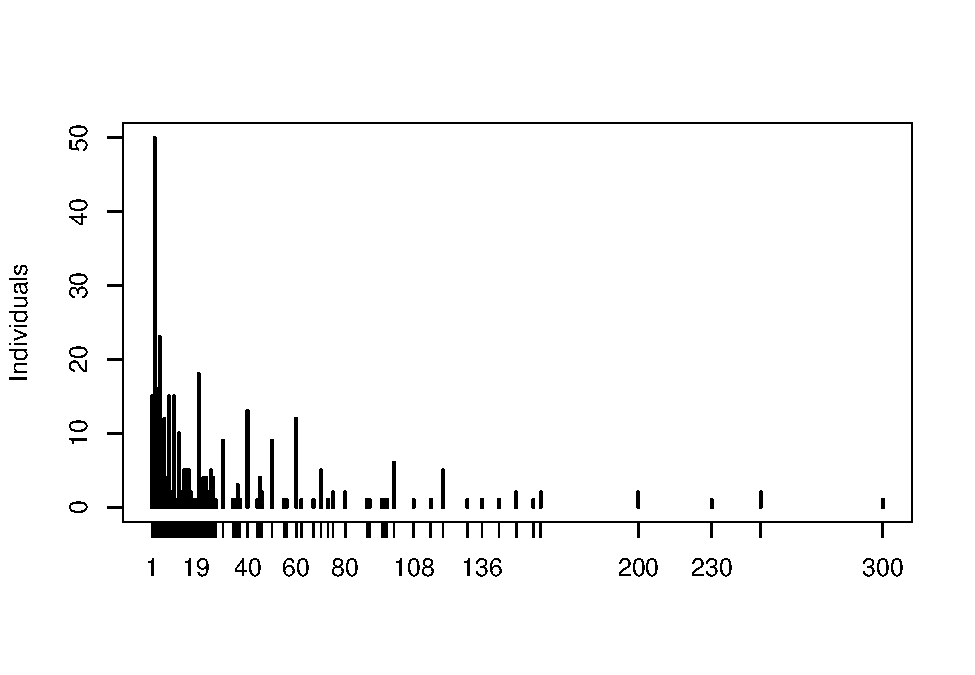
\includegraphics{Patagonia_parrots_density_analysis_files/figure-latex/unnamed-chunk-1-1} \caption{\textit{Enicognathus ferrugineus} count frequencies}\label{fig:unnamed-chunk-1}
\end{figure}

\section{\texorpdfstring{Austral parakeet \emph{Enicognathus
ferrugineus}}{Austral parakeet Enicognathus ferrugineus}}\label{austral-parakeet-enicognathus-ferrugineus}

\subsection{Estimating effective detection radius
(EDR)}\label{estimating-effective-detection-radius-edr}

We fit distance sampling models with detection predictor variables,
including the average group size, the number of groups that were
observed (to account for the possibility that grouping behaviour
influences detectability), and also habitat type. We used
forward-stepwise model selection, starting with single covariate models
and eliminating covariates that do not improve model parsimony
(i.e.~result in dAIC \textless{} 2) in relation to the null model.

\begin{longtable}[]{@{}lrrr@{}}
\caption{\textit{E. ferrugineous} EDR models AIC}\tabularnewline
\toprule
& df & AIC & dAIC\tabularnewline
\midrule
\endfirsthead
\toprule
& df & AIC & dAIC\tabularnewline
\midrule
\endhead
EDR.habitatype & 3 & 1434.532 & 0.00\tabularnewline
EDR.null & 1 & 1438.166 & 3.63\tabularnewline
EDR.avggroupsize & 2 & 1439.144 & 4.61\tabularnewline
EDR.numbergroups & 2 & 1440.166 & 5.63\tabularnewline
\bottomrule
\end{longtable}

The model (\texttt{EDR.habitatype}) has the lowest AIC (Table 1),
indicating that habitat type affects the effective detection radius
(EDR) of \emph{Enicognathus ferrugineus}. Specifically, detection radius
is higher in agropastoral than urban and other habitats (Table 2). This
means that detectability is higher in agropastoral habitats, and also
that the area surveyed in a given sample unit is larger if the habitat
therein is agropastoral vs.~urban or other, presubably because it is
possible to see further in pastures and planted fields than in forest or
urban environments.

\begin{longtable}[]{@{}lrrrr@{}}
\caption{\textit{E. ferrugineous} top-ranked EDR model
estimates}\tabularnewline
\toprule
& Estimate & Std. Error & z value &
Pr(\textgreater{}\textbar{}z\textbar{})\tabularnewline
\midrule
\endfirsthead
\toprule
& Estimate & Std. Error & z value &
Pr(\textgreater{}\textbar{}z\textbar{})\tabularnewline
\midrule
\endhead
log.tau\_(Intercept) & 4.589 & 0.038 & 119.365 & 0.000\tabularnewline
log.tau\_Urban & 0.057 & 0.058 & 0.988 & 0.323\tabularnewline
log.tau\_Agropastoral & 0.263 & 0.103 & 2.556 & 0.011\tabularnewline
\bottomrule
\end{longtable}

\begin{longtable}[]{@{}lr@{}}
\caption{\textit{E. ferrugineous} habitat-specific EDR
(m)}\tabularnewline
\toprule
Habitat & EDR\tabularnewline
\midrule
\endfirsthead
\toprule
Habitat & EDR\tabularnewline
\midrule
\endhead
Other & 98.36847\tabularnewline
Urban & 104.18432\tabularnewline
Agropastoral & 127.92056\tabularnewline
\bottomrule
\end{longtable}

\subsection{Models for number of
groups}\label{models-for-number-of-groups}

We then model the number of groups as a function of covariates. The
model for number of groups is G\textsubscript{i} \textasciitilde{}
Poisson(D\textsubscript{i}A\textsubscript{i}), where D\textsubscript{i}
= covariates and A\textsubscript{i} = area sampled in site \emph{i}.
A\textsubscript{i} is calculated using the habitat-specific estimated
EDR, and is added to the model as an offset.

\begin{figure}[H]
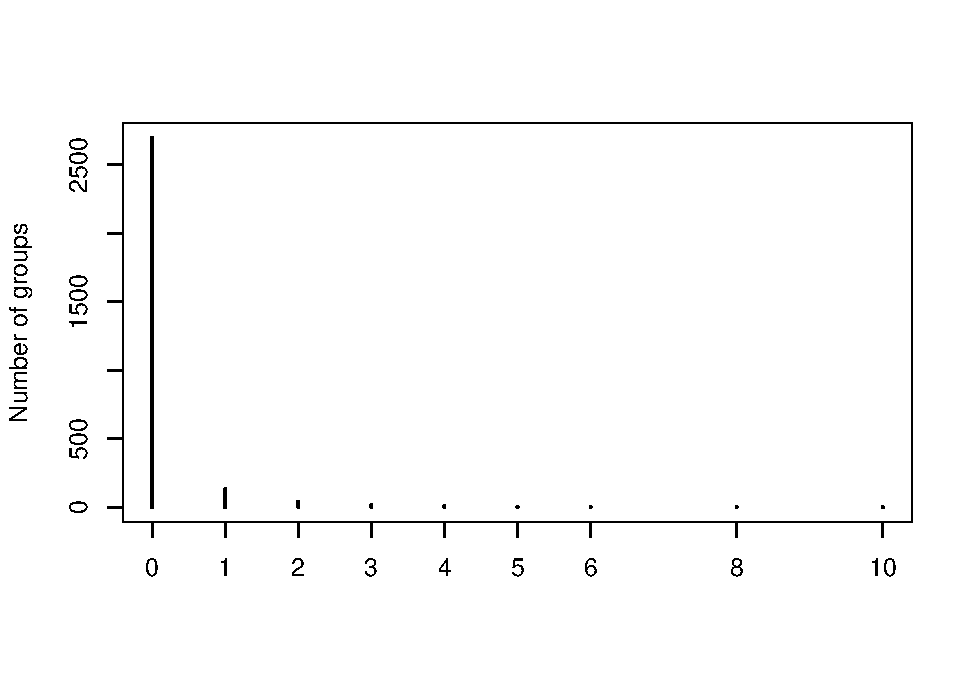
\includegraphics{Patagonia_parrots_density_analysis_files/figure-latex/unnamed-chunk-6-1} \caption{\textit{Enicognathus ferrugineus} group numbers }\label{fig:unnamed-chunk-6}
\end{figure}

\subsubsection{Model selection}\label{model-selection}

For number of groups, we use a stage-wise selection procedure. First, we
build a first set of models to evaluate the effect of covariates related
to habitat (habitat type and elevation).

\begin{longtable}[]{@{}lrrr@{}}
\caption{\textit{E. ferrugineous} number of group models}\tabularnewline
\toprule
& df & AIC & dAIC\tabularnewline
\midrule
\endfirsthead
\toprule
& df & AIC & dAIC\tabularnewline
\midrule
\endhead
ngroup.hab.ele2 & 5 & 2082.963 & 0.00\tabularnewline
ngroup.hab.ele & 4 & 2114.437 & 31.47\tabularnewline
ngroup.hab & 3 & 2133.717 & 50.75\tabularnewline
ngroup.ele2 & 3 & 2275.565 & 192.60\tabularnewline
ngroup.ele & 2 & 2323.806 & 240.84\tabularnewline
\bottomrule
\end{longtable}

The model with both habitat type and elevation (quadratic effect) has
the lowest AIC (Table 4), indicating that both covariates affect the
number of groups:

\begin{longtable}[]{@{}lrrrr@{}}
\caption{\textit{E. ferrugineous} `ngroup.hab.ele2' model
estimates}\tabularnewline
\toprule
& Estimate & Std. Error & z value &
Pr(\textgreater{}\textbar{}z\textbar{})\tabularnewline
\midrule
\endfirsthead
\toprule
& Estimate & Std. Error & z value &
Pr(\textgreater{}\textbar{}z\textbar{})\tabularnewline
\midrule
\endhead
(Intercept) & -3.108 & 0.233 & -13.356 & 0\tabularnewline
habitatOther & 1.507 & 0.202 & 7.455 & 0\tabularnewline
habitatUrban & 2.390 & 0.202 & 11.823 & 0\tabularnewline
elevation & -0.004 & 0.001 & -7.032 & 0\tabularnewline
I(elevation\^{}2) & 0.000 & 0.000 & 5.947 & 0\tabularnewline
\bottomrule
\end{longtable}

\begin{longtable}[]{@{}lrrrr@{}}
\caption{Deviance partitioning of `ngroup.hab.ele2' model for
\textit{E. ferrugineous}}\tabularnewline
\toprule
& Df & Deviance & Resid. Df & Resid. Dev\tabularnewline
\midrule
\endfirsthead
\toprule
& Df & Deviance & Resid. Df & Resid. Dev\tabularnewline
\midrule
\endhead
NULL & NA & NA & 2900 & 1865.338\tabularnewline
habitat & 2 & 207.965 & 2898 & 1657.373\tabularnewline
elevation & 1 & 21.279 & 2897 & 1636.094\tabularnewline
I(elevation\^{}2) & 1 & 33.475 & 2896 & 1602.619\tabularnewline
\bottomrule
\end{longtable}

We then proceed by adding within-year temporal covariates
(breeding/non-breeding season and julian date) and their interactions
with habitat.

\begin{longtable}[]{@{}lrrr@{}}
\caption{\textit{E. ferrugineous} number of group models (within-year
temporal predictors) AIC}\tabularnewline
\toprule
& df & AIC & dAIC\tabularnewline
\midrule
\endfirsthead
\toprule
& df & AIC & dAIC\tabularnewline
\midrule
\endhead
ngroup.habXseason.ele2 & 8 & 2065.594 & 0.00\tabularnewline
ngroup.hab.season.ele2 & 6 & 2067.555 & 1.96\tabularnewline
ngroup.habXjdate.ele2 & 8 & 2081.546 & 15.95\tabularnewline
ngroup.hab.ele2 & 5 & 2082.963 & 17.37\tabularnewline
ngroup.hab.jdate.ele2 & 6 & 2084.491 & 18.90\tabularnewline
\bottomrule
\end{longtable}

The model with the season*habitat interaction (Table 8) is equally
parcimonious with the model with only the additive effects (Table 9).
Given these are nested models, this indicates the interaction only
marginally improves the model fit, so will continue with model with
season and no interaction:

\begin{longtable}[]{@{}lrrrr@{}}
\caption{\textit{E. ferrugineous} `ngroup.habXseason.ele2' interaction
model estimates}\tabularnewline
\toprule
& Estimate & Std. Error & z value &
Pr(\textgreater{}\textbar{}z\textbar{})\tabularnewline
\midrule
\endfirsthead
\toprule
& Estimate & Std. Error & z value &
Pr(\textgreater{}\textbar{}z\textbar{})\tabularnewline
\midrule
\endhead
(Intercept) & -18.187 & 558.012 & -0.033 & 0.974\tabularnewline
elevation & -0.004 & 0.001 & -6.547 & 0.000\tabularnewline
I(elevation\^{}2) & 0.000 & 0.000 & 5.500 & 0.000\tabularnewline
habitatOther & 15.797 & 558.012 & 0.028 & 0.977\tabularnewline
habitatUrban & 2.008 & 908.375 & 0.002 & 0.998\tabularnewline
seasonnon-breeding & 15.186 & 558.012 & 0.027 & 0.978\tabularnewline
habitatOther:seasonnon-breeding & -14.357 & 558.012 & -0.026 &
0.979\tabularnewline
habitatUrban:seasonnon-breeding & 0.266 & 908.375 & 0.000 &
1.000\tabularnewline
\bottomrule
\end{longtable}

\begin{longtable}[]{@{}lrrrr@{}}
\caption{\textit{E. ferrugineous} `ngroup.hab.season.ele2' additive
model estimates}\tabularnewline
\toprule
& Estimate & Std. Error & z value &
Pr(\textgreater{}\textbar{}z\textbar{})\tabularnewline
\midrule
\endfirsthead
\toprule
& Estimate & Std. Error & z value &
Pr(\textgreater{}\textbar{}z\textbar{})\tabularnewline
\midrule
\endhead
(Intercept) & -4.250 & 0.412 & -10.318 & 0.000\tabularnewline
habitatOther & 1.510 & 0.204 & 7.411 & 0.000\tabularnewline
habitatUrban & 2.314 & 0.203 & 11.424 & 0.000\tabularnewline
elevation & -0.004 & 0.001 & -6.408 & 0.000\tabularnewline
I(elevation\^{}2) & 0.000 & 0.000 & 5.365 & 0.000\tabularnewline
seasonnon-breeding & 1.175 & 0.340 & 3.451 & 0.001\tabularnewline
\bottomrule
\end{longtable}

Finally, we assess year effects by adding a year covariate (2013-2016).

\begin{longtable}[]{@{}lrrr@{}}
\caption{\textit{E. ferrugineous} number of group models (year
predictor) AIC table}\tabularnewline
\toprule
& df & AIC & dAIC\tabularnewline
\midrule
\endfirsthead
\toprule
& df & AIC & dAIC\tabularnewline
\midrule
\endhead
ngroup.hab.season.ele2.year & 9 & 2022.265 & 0.00\tabularnewline
ngroup.hab.season.ele2 & 6 & 2067.555 & 45.29\tabularnewline
\bottomrule
\end{longtable}

The model with lowest AIC indicates that the number of groups is
affected by habitat ype, elevation, season (breeding/non breeding) and
year.

\begin{longtable}[]{@{}lrrrr@{}}
\caption{\textit{E. ferrugineous} top-ranked
(ngroup.hab.season.ele2.year) model estimates}\tabularnewline
\toprule
& Estimate & Std. Error & z value &
Pr(\textgreater{}\textbar{}z\textbar{})\tabularnewline
\midrule
\endfirsthead
\toprule
& Estimate & Std. Error & z value &
Pr(\textgreater{}\textbar{}z\textbar{})\tabularnewline
\midrule
\endhead
(Intercept) & -4.716 & 0.417 & -11.311 & 0.000\tabularnewline
habitatOther & 1.739 & 0.206 & 8.434 & 0.000\tabularnewline
habitatUrban & 2.460 & 0.204 & 12.075 & 0.000\tabularnewline
elevation & -0.003 & 0.001 & -5.712 & 0.000\tabularnewline
I(elevation\^{}2) & 0.000 & 0.000 & 4.588 & 0.000\tabularnewline
seasonnon-breeding & 1.022 & 0.348 & 2.939 & 0.003\tabularnewline
as.factor(year)2014 & 0.092 & 0.168 & 0.549 & 0.583\tabularnewline
as.factor(year)2015 & 0.918 & 0.161 & 5.688 & 0.000\tabularnewline
as.factor(year)2016 & 0.612 & 0.205 & 2.979 & 0.003\tabularnewline
\bottomrule
\end{longtable}

\begin{longtable}[]{@{}lrrrr@{}}
\caption{Deviance partitioning of top-ranked
`ngroup.hab.season.ele2.year' model for
\textit{E. ferrugineous}}\tabularnewline
\toprule
& Df & Deviance & Resid. Df & Resid. Dev\tabularnewline
\midrule
\endfirsthead
\toprule
& Df & Deviance & Resid. Df & Resid. Dev\tabularnewline
\midrule
\endhead
NULL & NA & NA & 2900 & 1865.338\tabularnewline
habitat & 2 & 207.965 & 2898 & 1657.373\tabularnewline
elevation & 1 & 21.279 & 2897 & 1636.094\tabularnewline
I(elevation\^{}2) & 1 & 33.475 & 2896 & 1602.619\tabularnewline
season & 1 & 17.408 & 2895 & 1585.211\tabularnewline
as.factor(year) & 3 & 51.290 & 2892 & 1533.921\tabularnewline
\bottomrule
\end{longtable}

\subsection{Models for group size}\label{models-for-group-size}

The count distribution is characterized with a spike at 2 (Figure 1),
and by the absence of 0s due to group size being conditional on having
\textgreater{}0 birds to consider it a group.

We start developing a general V-Inflated Poisson (VIP) model (``V''
stands for ``variable''``, in refence to the''Z" representing 0 in a
zero-inflated Poisson model, or ZIP), then we add the \textgreater{}0
condition.

R functions for the VIP model are presented at the end of this document,
including simulations to check the estimating procedure.

\subsubsection{Maximum likelihood}\label{maximum-likelihood}

Let \(Y\) be a random variable, and \(y\) are observations, \(V\) is the
count value that has some extra probability mass (\(V=0\) is the ZIP
model), \(f(y; \lambda)\) is the Poisson density
(\(f(y; \lambda) = e^{-\lambda} \frac{\lambda^{y}}{y!}\)).

The V-Inflated density can be written as
\(P(Y=y) = \phi I(Y=V) + (1-\phi) f(y; \lambda)\) which is
\(\phi + (1-\phi) f(V; \lambda)\) when \(Y=V\) and
\((1-\phi) f(y; \lambda)\) otherwise.

We define the extra probability mass at \(V=2\) to account for the group
size peak in pairs. The model is also truncated at 0, because there are
no groups with 0 individuals. We include habitat type as a covariate for
the count (Poisson) component, and compare models with and without
season (breeding/non-breeding) as a covariate for the V-inflation
probability.

\begin{longtable}[]{@{}lrrrr@{}}
\caption{\textit{E. ferrugineous} group size model
estimates}\tabularnewline
\toprule
& Estimate & Std. Error & z value &
Pr(\textgreater{}\textbar{}z\textbar{})\tabularnewline
\midrule
\endfirsthead
\toprule
& Estimate & Std. Error & z value &
Pr(\textgreater{}\textbar{}z\textbar{})\tabularnewline
\midrule
\endhead
P\_(Intercept) & 1.000 & 0.019 & 52.686 & 0.000\tabularnewline
P\_Urban & 1.754 & 0.023 & 76.483 & 0.000\tabularnewline
P\_Agropastoral & 0.612 & 0.037 & 16.744 & 0.000\tabularnewline
V\_(Intercept) & 1.316 & 0.816 & 1.612 & 0.107\tabularnewline
V\_seasonnon-breeding & -3.474 & 0.839 & -4.142 & 0.000\tabularnewline
\bottomrule
\end{longtable}

Estimated model coefficients (Table 13) indicate that group sizes are
larger in urban (\(\beta\) = 1.754) and agropastoral (\(\beta\) = 1.754)
habitats when compared to other natural habitats. Moreover, the
probability of there being extra pairs (i.e.~the V-inflation
probability, \(\phi\)) is smaller in the non-breeding season (\(\beta\)
= 1.754).

Considence intervals (CI) based on estimated standard errors can be
obtained (Table 14):

\begin{longtable}[]{@{}lrr@{}}
\caption{\textit{E. ferrugineous} group size model CI}\tabularnewline
\toprule
& 2.5\% & 97.5\%\tabularnewline
\midrule
\endfirsthead
\toprule
& 2.5\% & 97.5\%\tabularnewline
\midrule
\endhead
P\_(Intercept) & 0.963 & 1.037\tabularnewline
P\_Urban & 1.709 & 1.799\tabularnewline
P\_Agropastoral & 0.540 & 0.683\tabularnewline
V\_(Intercept) & -0.284 & 2.915\tabularnewline
V\_seasonnon-breeding & -5.118 & -1.830\tabularnewline
\bottomrule
\end{longtable}

Alternatively, we can estimate confidence intervals based on quantiles
using bootstrap samples (with n=250) for the estimated coefficients
(Table 15).

\begin{longtable}[]{@{}lrrr@{}}
\caption{Estimated coefficients and 95\% CI based on bootstrap sample
(n= 250) quantiles for \textit{E. ferrugineous} group size
models}\tabularnewline
\toprule
& Estimate & 2.5\% & 97.5\%\tabularnewline
\midrule
\endfirsthead
\toprule
& Estimate & 2.5\% & 97.5\%\tabularnewline
\midrule
\endhead
P\_(Intercept) & 1.000 & -20.137 & 28.356\tabularnewline
P\_Urban & 1.754 & -19.089 & 23.699\tabularnewline
P\_Agropastoral & 0.612 & -18.971 & 23.497\tabularnewline
V\_(Intercept) & 1.316 & -19.202 & 21.600\tabularnewline
V\_seasonnon-breeding & -3.474 & -20.430 & 20.669\tabularnewline
\bottomrule
\end{longtable}

\begin{center}\rule{0.5\linewidth}{\linethickness}\end{center}

\section{\texorpdfstring{Slender-billed parakeet \emph{Enicognathus
leptorhynchus}}{Slender-billed parakeet Enicognathus leptorhynchus}}\label{slender-billed-parakeet-enicognathus-leptorhynchus}

\begin{figure}[H]
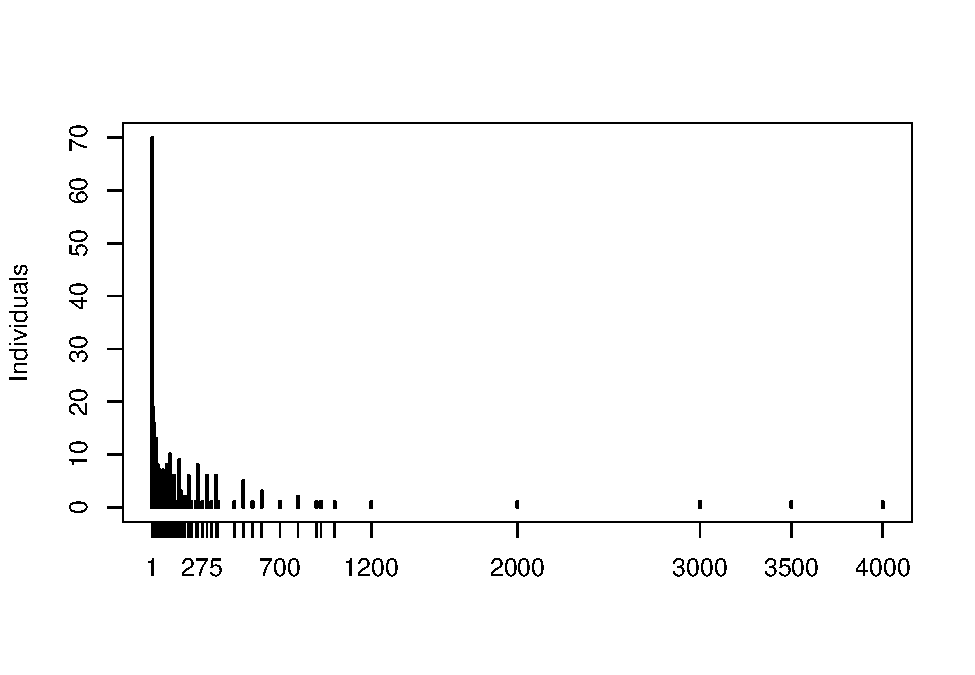
\includegraphics{Patagonia_parrots_density_analysis_files/figure-latex/unnamed-chunk-18-1} \caption{\textit{Enicognathus leptorhynchus} count frequencies}\label{fig:unnamed-chunk-18}
\end{figure}

\subsection{Estimating effective detection radius
(EDR)}\label{estimating-effective-detection-radius-edr-1}

We follow the same procedure used for the austral parakeet above.

\begin{longtable}[]{@{}lrrr@{}}
\caption{\textit{E. leptorhynchus} EDR models AIC}\tabularnewline
\toprule
& df & AIC & dAIC\tabularnewline
\midrule
\endfirsthead
\toprule
& df & AIC & dAIC\tabularnewline
\midrule
\endhead
EDR.avggroupsize.habitat & 4 & 1054.464 & 0.00\tabularnewline
EDR.habitat.avggroupsize.numbergroups & 5 & 1059.062 &
4.60\tabularnewline
EDR.avggroupsize & 2 & 1063.875 & 9.41\tabularnewline
EDR.avggroupsize.numbergroups & 3 & 1064.553 & 10.09\tabularnewline
EDR.habitat.numbergroups & 4 & 1069.376 & 14.91\tabularnewline
EDR.habitatype & 3 & 1070.755 & 16.29\tabularnewline
EDR.null & 1 & 1086.330 & 31.87\tabularnewline
EDR.numbergroups & 2 & 1087.172 & 32.71\tabularnewline
\bottomrule
\end{longtable}

The model (\texttt{EDR.avggroupsize.habitat}) has the lowest AIC (Table
16), indicating that habitat type and average group size affect the
effective detection radius (EDR) of \emph{Enicognathus leptorhynchus}.
The mean EDR for each habitat, predicted using model coefficients and
the habitat-specific means of average group size, is shown in Table 17.

\begin{longtable}[]{@{}lrrrr@{}}
\caption{\textit{E. leptorhynchus} top-ranked EDR model
estimates}\tabularnewline
\toprule
& Estimate & Std. Error & z value &
Pr(\textgreater{}\textbar{}z\textbar{})\tabularnewline
\midrule
\endfirsthead
\toprule
& Estimate & Std. Error & z value &
Pr(\textgreater{}\textbar{}z\textbar{})\tabularnewline
\midrule
\endhead
log.tau\_(Intercept) & 5.361 & 0 & 1.273654e+51 & 0\tabularnewline
log.tau\_gavg & 0.001 & 0 & 9.610881e+50 & 0\tabularnewline
log.tau\_Urban & -0.266 & 0 & -6.308165e+49 & 0\tabularnewline
log.tau\_Agropastoral & -0.029 & 0 & -4.843080e+48 & 0\tabularnewline
\bottomrule
\end{longtable}

\begin{longtable}[]{@{}lr@{}}
\caption{\textit{E. leptorhynchus} habitat-specific mean EDR
(m)}\tabularnewline
\toprule
Habitat & EDR\tabularnewline
\midrule
\endfirsthead
\toprule
Habitat & EDR\tabularnewline
\midrule
\endhead
Other & 235.4183\tabularnewline
Urban & 224.2124\tabularnewline
Agropastoral & 180.7002\tabularnewline
\bottomrule
\end{longtable}

\subsection{Models for number of
groups}\label{models-for-number-of-groups-1}

As for the austral parakeet, the model for number of groups is
G\textsubscript{i} \textasciitilde{}
Poisson(D\textsubscript{i}A\textsubscript{i}), where D\textsubscript{i}
= covariates and A\textsubscript{i} = area sampled in site \emph{i}.
A\textsubscript{i} is calculated using the habitat-specific estimated
EDR, and is added to the model as an offset.

\begin{figure}[H]
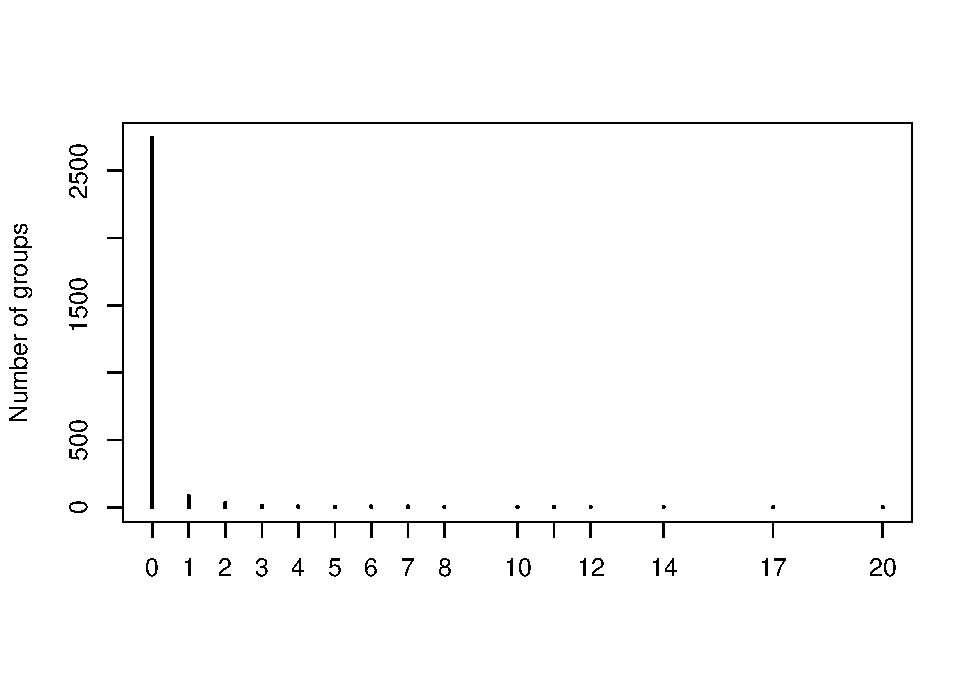
\includegraphics{Patagonia_parrots_density_analysis_files/figure-latex/unnamed-chunk-22-1} \caption{\textit{Enicognathus leptorhynchus} group numbers }\label{fig:unnamed-chunk-22}
\end{figure}

\subsubsection{Model selection}\label{model-selection-1}

First set of models to evaluate the effect of habitat type and elevation
covariates (Table 18):

\begin{longtable}[]{@{}lrrr@{}}
\caption{\textit{E. leptorhynchus} number of group
models}\tabularnewline
\toprule
& df & AIC & dAIC\tabularnewline
\midrule
\endfirsthead
\toprule
& df & AIC & dAIC\tabularnewline
\midrule
\endhead
ngroup.hab.ele2 & 5 & 2486.990 & 0.00\tabularnewline
ngroup.hab.ele & 4 & 2487.834 & 0.84\tabularnewline
ngroup.hab & 3 & 2493.346 & 6.36\tabularnewline
ngroup.ele2 & 3 & 2746.031 & 259.04\tabularnewline
ngroup.ele & 2 & 2761.122 & 274.13\tabularnewline
\bottomrule
\end{longtable}

The models `ngroup.hab.ele' (with linear elevation effect) and
`ngroup.hab.ele2' (with quadratic effect) are equally parsimonious
(Table 18), but the quadratic term in the latter is mostly uniformative
(Tables 19-20). Given these are nested models, we drop the quadratic
term and continue with the model with habitat and linear elevation
effects.

\begin{longtable}[]{@{}lrrrr@{}}
\caption{\textit{E. leptorhynchus} `ngroup.hab.ele' model
estimates}\tabularnewline
\toprule
& Estimate & Std. Error & z value &
Pr(\textgreater{}\textbar{}z\textbar{})\tabularnewline
\midrule
\endfirsthead
\toprule
& Estimate & Std. Error & z value &
Pr(\textgreater{}\textbar{}z\textbar{})\tabularnewline
\midrule
\endhead
(Intercept) & -2.781 & 0.123 & -22.568 & 0.000\tabularnewline
habitatOther & -2.035 & 0.147 & -13.874 & 0.000\tabularnewline
habitatUrban & -0.734 & 0.143 & -5.116 & 0.000\tabularnewline
elevation & 0.000 & 0.000 & 2.736 & 0.006\tabularnewline
\bottomrule
\end{longtable}

\begin{longtable}[]{@{}lrrrr@{}}
\caption{Deviance partitioning of `ngroup.hab.ele' model for
\textit{E. leptorhynchus}}\tabularnewline
\toprule
& Df & Deviance & Resid. Df & Resid. Dev\tabularnewline
\midrule
\endfirsthead
\toprule
& Df & Deviance & Resid. Df & Resid. Dev\tabularnewline
\midrule
\endhead
NULL & NA & NA & 2900 & 2358.856\tabularnewline
habitat & 2 & 270.326 & 2898 & 2088.530\tabularnewline
elevation & 1 & 7.512 & 2897 & 2081.018\tabularnewline
\bottomrule
\end{longtable}

Adding within-year temporal covariates (breeding/non-breeding season and
julian date) and their interactions with habitat:

\begin{longtable}[]{@{}lrrr@{}}
\caption{\textit{E. leptorhynchus} number of group models (within-year
temporal predictors) AIC}\tabularnewline
\toprule
& df & AIC & dAIC\tabularnewline
\midrule
\endfirsthead
\toprule
& df & AIC & dAIC\tabularnewline
\midrule
\endhead
ngroup.habXjdate.ele & 7 & 2110.653 & 0.00\tabularnewline
ngroup.hab.ele.jdate & 5 & 2230.345 & 119.69\tabularnewline
ngroup.habXseason.ele & 7 & 2472.731 & 362.08\tabularnewline
ngroup.hab.ele & 4 & 2487.834 & 377.18\tabularnewline
ngroup.hab.ele.season & 5 & 2489.059 & 378.41\tabularnewline
\bottomrule
\end{longtable}

The model `ngroup.habXjdate.ele' has the lowest AIC (Table 21).

\begin{longtable}[]{@{}lrrrr@{}}
\caption{\textit{E. leptorhynchus} `ngroup.habXjdate.ele' model
estimates}\tabularnewline
\toprule
& Estimate & Std. Error & z value &
Pr(\textgreater{}\textbar{}z\textbar{})\tabularnewline
\midrule
\endfirsthead
\toprule
& Estimate & Std. Error & z value &
Pr(\textgreater{}\textbar{}z\textbar{})\tabularnewline
\midrule
\endhead
(Intercept) & -1.463 & 0.167 & -8.741 & 0.000\tabularnewline
elevation & 0.000 & 0.000 & 1.939 & 0.053\tabularnewline
habitatOther & 2.234 & 0.590 & 3.788 & 0.000\tabularnewline
habitatUrban & 0.412 & 0.310 & 1.329 & 0.184\tabularnewline
jdate & -0.006 & 0.001 & -10.029 & 0.000\tabularnewline
habitatOther:jdate & -0.040 & 0.007 & -5.589 & 0.000\tabularnewline
habitatUrban:jdate & -0.009 & 0.002 & -4.095 & 0.000\tabularnewline
\bottomrule
\end{longtable}

Finally, we assess year effects by adding a year covariate (2013-2016).

\begin{longtable}[]{@{}lrrr@{}}
\caption{\textit{E. leptorhynchus} number of group models (year
predictor) AIC table}\tabularnewline
\toprule
& df & AIC & dAIC\tabularnewline
\midrule
\endfirsthead
\toprule
& df & AIC & dAIC\tabularnewline
\midrule
\endhead
ngroup.habXjdate.ele.year & 8 & 1993.981 & 0.00\tabularnewline
ngroup.habXjdate.ele & 7 & 2110.653 & 116.67\tabularnewline
\bottomrule
\end{longtable}

The best-ranked model indicates that the number of groups is affected by
habitat type, elevation, julian date and year (Tables 23-24).

\begin{longtable}[]{@{}lrrrr@{}}
\caption{\textit{E. leptorhynchus} `ngroup.habXjdate.ele.year' model
estimates}\tabularnewline
\toprule
& Estimate & Std. Error & z value &
Pr(\textgreater{}\textbar{}z\textbar{})\tabularnewline
\midrule
\endfirsthead
\toprule
& Estimate & Std. Error & z value &
Pr(\textgreater{}\textbar{}z\textbar{})\tabularnewline
\midrule
\endhead
(Intercept) & -3.952 & 0.264 & -14.974 & 0.000\tabularnewline
habitatOther & -1.629 & 0.150 & -10.893 & 0.000\tabularnewline
habitatUrban & -0.506 & 0.144 & -3.507 & 0.000\tabularnewline
elevation & 0.000 & 0.000 & 2.851 & 0.004\tabularnewline
seasonnon-breeding & -0.749 & 0.201 & -3.723 & 0.000\tabularnewline
as.factor(year)2014 & 0.669 & 0.276 & 2.422 & 0.015\tabularnewline
as.factor(year)2015 & 1.763 & 0.237 & 7.452 & 0.000\tabularnewline
as.factor(year)2016 & 3.280 & 0.239 & 13.705 & 0.000\tabularnewline
\bottomrule
\end{longtable}

\begin{longtable}[]{@{}lrrrr@{}}
\caption{Deviance partitioning of `ngroup.habXjdate.ele.year' model for
\textit{E. leptorhynchus}}\tabularnewline
\toprule
& Df & Deviance & Resid. Df & Resid. Dev\tabularnewline
\midrule
\endfirsthead
\toprule
& Df & Deviance & Resid. Df & Resid. Dev\tabularnewline
\midrule
\endhead
NULL & NA & NA & 2900 & 2358.856\tabularnewline
habitat & 2 & 270.326 & 2898 & 2088.530\tabularnewline
elevation & 1 & 7.512 & 2897 & 2081.018\tabularnewline
season & 1 & 0.776 & 2896 & 2080.243\tabularnewline
as.factor(year) & 3 & 501.078 & 2893 & 1579.165\tabularnewline
\bottomrule
\end{longtable}

\subsection{Models for group size}\label{models-for-group-size-1}

\begin{longtable}[]{@{}lrrrr@{}}
\caption{\textit{E. leptorhynchus} group size model
estimates}\tabularnewline
\toprule
& Estimate & Std. Error & z value &
Pr(\textgreater{}\textbar{}z\textbar{})\tabularnewline
\midrule
\endfirsthead
\toprule
& Estimate & Std. Error & z value &
Pr(\textgreater{}\textbar{}z\textbar{})\tabularnewline
\midrule
\endhead
P\_(Intercept) & 9.348 & NA & NA & NA\tabularnewline
P\_Urban & 4.168 & NA & NA & NA\tabularnewline
P\_Agropastoral & -7.553 & NA & NA & NA\tabularnewline
V\_(Intercept) & -0.008 & NA & NA & NA\tabularnewline
V\_seasonnon-breeding & -10.208 & NA & NA & NA\tabularnewline
\bottomrule
\end{longtable}

Model-fitting function cannot estimate coefficient standard errors due
to sigular Hessian matrix (Table 25). We can calculate confidence
intervals based on quantiles using bootstrap (with n=250):

\begin{longtable}[]{@{}lrrr@{}}
\caption{Estimated coefficients and 95\% CI based on bootstrap quantiles
for \textit{E. leptorhynchus} group size models}\tabularnewline
\toprule
& Estimate & 2.5\% & 97.5\%\tabularnewline
\midrule
\endfirsthead
\toprule
& Estimate & 2.5\% & 97.5\%\tabularnewline
\midrule
\endhead
P\_(Intercept) & 9.348 & -20.918 & 30.698\tabularnewline
P\_Urban & 4.168 & -26.730 & 26.184\tabularnewline
P\_Agropastoral & -7.553 & -25.738 & 25.361\tabularnewline
V\_(Intercept) & -0.008 & -24.252 & 25.802\tabularnewline
V\_seasonnon-breeding & -10.208 & -25.553 & 27.833\tabularnewline
\bottomrule
\end{longtable}

\begin{center}\rule{0.5\linewidth}{\linethickness}\end{center}

\section{VIP model - R functions and
simulations}\label{vip-model---r-functions-and-simulations}

\subsubsection{Peter Sólymos}\label{peter-solymos}

\begin{Shaded}
\begin{Highlighting}[]
\NormalTok{vip <-}
\ControlFlowTok{function}\NormalTok{(Y, X, Z, }\DataTypeTok{V=}\DecValTok{0}\NormalTok{,}
\NormalTok{offsetx, offsetz, weights, }\DataTypeTok{linkz=}\StringTok{"logit"}\NormalTok{,}
\DataTypeTok{truncate=}\OtherTok{FALSE}\NormalTok{, }\DataTypeTok{hessian=}\OtherTok{TRUE}\NormalTok{, }\DataTypeTok{method=}\StringTok{"Nelder-Mead"}\NormalTok{, }\DataTypeTok{init=}\OtherTok{NULL}\NormalTok{, ...) \{}
    \ControlFlowTok{if}\NormalTok{ (}\KeywordTok{missing}\NormalTok{(Y))}
        \KeywordTok{stop}\NormalTok{(}\StringTok{"C'mon, you must have some data?!"}\NormalTok{)}
    \ControlFlowTok{if}\NormalTok{ (truncate }\OperatorTok{&&}\StringTok{ }\KeywordTok{any}\NormalTok{(Y }\OperatorTok{<}\StringTok{ }\DecValTok{1}\NormalTok{))}
        \KeywordTok{stop}\NormalTok{(}\StringTok{"Y must be >0 when truncate=TRUE"}\NormalTok{)}
\NormalTok{    n <-}\StringTok{ }\KeywordTok{length}\NormalTok{(Y)}
\NormalTok{    id0 <-}\StringTok{ }\NormalTok{Y }\OperatorTok{==}\StringTok{ }\NormalTok{V}
\NormalTok{    id1 <-}\StringTok{ }\OperatorTok{!}\NormalTok{id0}
    \ControlFlowTok{if}\NormalTok{ (}\KeywordTok{missing}\NormalTok{(X)) \{}
\NormalTok{        X <-}\StringTok{ }\KeywordTok{matrix}\NormalTok{(}\DecValTok{1}\NormalTok{, n, }\DecValTok{1}\NormalTok{)}
        \KeywordTok{colnames}\NormalTok{(X) <-}\StringTok{ "(Intercept)"}
\NormalTok{    \}}
    \ControlFlowTok{if}\NormalTok{ (}\KeywordTok{missing}\NormalTok{(Z)) \{}
\NormalTok{        Z <-}\StringTok{ }\KeywordTok{matrix}\NormalTok{(}\DecValTok{1}\NormalTok{, n, }\DecValTok{1}\NormalTok{)}
        \KeywordTok{colnames}\NormalTok{(Z) <-}\StringTok{ "(Intercept)"}
\NormalTok{    \}}
\NormalTok{    kx <-}\StringTok{ }\KeywordTok{ncol}\NormalTok{(X)}
\NormalTok{    kz <-}\StringTok{ }\KeywordTok{ncol}\NormalTok{(Z)}
    \ControlFlowTok{if}\NormalTok{ (}\KeywordTok{missing}\NormalTok{(offsetx))}
\NormalTok{        offsetx <-}\StringTok{ }\DecValTok{0}
    \ControlFlowTok{if}\NormalTok{ (}\KeywordTok{missing}\NormalTok{(offsetz))}
\NormalTok{        offsetz <-}\StringTok{ }\DecValTok{0}
    \ControlFlowTok{if}\NormalTok{ (}\KeywordTok{missing}\NormalTok{(weights))}
\NormalTok{        weights <-}\StringTok{ }\KeywordTok{rep}\NormalTok{(}\DecValTok{1}\NormalTok{, n)}
\NormalTok{    linkinvx <-}\StringTok{ }\KeywordTok{poisson}\NormalTok{(}\StringTok{"log"}\NormalTok{)}\OperatorTok{$}\NormalTok{linkinv}
\NormalTok{    linkinvz <-}\StringTok{ }\KeywordTok{binomial}\NormalTok{(linkz)}\OperatorTok{$}\NormalTok{linkinv}
\NormalTok{    good.num.limit <-}\StringTok{ }\KeywordTok{c}\NormalTok{(.Machine}\OperatorTok{$}\NormalTok{double.xmin, .Machine}\OperatorTok{$}\NormalTok{double.xmax)}\OperatorTok{^}\NormalTok{(}\DecValTok{1}\OperatorTok{/}\DecValTok{3}\NormalTok{)}

\NormalTok{    ## VIP model full likelihood}
\NormalTok{    nll_VIP_ML <-}\StringTok{ }\ControlFlowTok{function}\NormalTok{(parms) \{}
\NormalTok{        mu <-}\StringTok{ }\KeywordTok{as.vector}\NormalTok{(}\KeywordTok{linkinvx}\NormalTok{(X }\OperatorTok\StringTok{ }\NormalTok{parms[}\DecValTok{1}\OperatorTok{:}\NormalTok{kx] }\OperatorTok{+}\StringTok{ }\NormalTok{offsetx))}
\NormalTok{        phi <-}\StringTok{ }\KeywordTok{as.vector}\NormalTok{(}\KeywordTok{linkinvz}\NormalTok{(Z }\OperatorTok\StringTok{ }\NormalTok{parms[(kx }\OperatorTok{+}\StringTok{ }\DecValTok{1}\NormalTok{)}\OperatorTok{:}\NormalTok{(kx }\OperatorTok{+}\StringTok{ }\NormalTok{kz)] }\OperatorTok{+}\StringTok{ }\NormalTok{offsetz))}
\NormalTok{        loglik0 <-}\StringTok{ }\KeywordTok{log}\NormalTok{(phi }\OperatorTok{+}\StringTok{ }\NormalTok{(}\DecValTok{1} \OperatorTok{-}\StringTok{ }\NormalTok{phi) }\OperatorTok{*}\StringTok{ }\KeywordTok{dpois}\NormalTok{(V, }\DataTypeTok{lambda =}\NormalTok{ mu, }\DataTypeTok{log =} \OtherTok{FALSE}\NormalTok{))}
\NormalTok{        loglik1 <-}\StringTok{ }\KeywordTok{log}\NormalTok{(}\DecValTok{1} \OperatorTok{-}\StringTok{ }\NormalTok{phi) }\OperatorTok{+}\StringTok{ }\KeywordTok{dpois}\NormalTok{(Y, }\DataTypeTok{lambda =}\NormalTok{ mu, }\DataTypeTok{log =} \OtherTok{TRUE}\NormalTok{)}
\NormalTok{        loglik <-}\StringTok{ }\KeywordTok{sum}\NormalTok{(weights[id0] }\OperatorTok{*}\StringTok{ }\NormalTok{loglik0[id0]) }\OperatorTok{+}\StringTok{ }\KeywordTok{sum}\NormalTok{(weights[id1] }\OperatorTok{*}\StringTok{ }\NormalTok{loglik1[id1])}
        \ControlFlowTok{if}\NormalTok{ (}\OperatorTok{!}\KeywordTok{is.finite}\NormalTok{(loglik) }\OperatorTok{||}\StringTok{ }\KeywordTok{is.na}\NormalTok{(loglik))}
\NormalTok{            loglik <-}\StringTok{ }\OperatorTok{-}\NormalTok{good.num.limit[}\DecValTok{2}\NormalTok{]}
        \OperatorTok{-}\NormalTok{loglik}
\NormalTok{    \}}
\NormalTok{    ## 0-truncated VIP model full likelihood}
\NormalTok{    nll_VIP_TR <-}\StringTok{ }\ControlFlowTok{function}\NormalTok{(parms) \{}
\NormalTok{        mu <-}\StringTok{ }\KeywordTok{as.vector}\NormalTok{(}\KeywordTok{linkinvx}\NormalTok{(X }\OperatorTok\StringTok{ }\NormalTok{parms[}\DecValTok{1}\OperatorTok{:}\NormalTok{kx] }\OperatorTok{+}\StringTok{ }\NormalTok{offsetx))}
\NormalTok{        phi <-}\StringTok{ }\KeywordTok{as.vector}\NormalTok{(}\KeywordTok{linkinvz}\NormalTok{(Z }\OperatorTok\StringTok{ }\NormalTok{parms[(kx }\OperatorTok{+}\StringTok{ }\DecValTok{1}\NormalTok{)}\OperatorTok{:}\NormalTok{(kx }\OperatorTok{+}\StringTok{ }\NormalTok{kz)] }\OperatorTok{+}\StringTok{ }\NormalTok{offsetz))}
\NormalTok{        loglik0 <-}\StringTok{ }\KeywordTok{log}\NormalTok{(phi }\OperatorTok{+}\StringTok{ }\NormalTok{(}\DecValTok{1} \OperatorTok{-}\StringTok{ }\NormalTok{phi) }\OperatorTok{*}\StringTok{ }\KeywordTok{dpois}\NormalTok{(V, }\DataTypeTok{lambda =}\NormalTok{ mu, }\DataTypeTok{log =} \OtherTok{FALSE}\NormalTok{) }\OperatorTok{/}\StringTok{ }\NormalTok{(}\DecValTok{1}\OperatorTok{-}\KeywordTok{exp}\NormalTok{(}\OperatorTok{-}\NormalTok{mu)))}
\NormalTok{        loglik1 <-}\StringTok{ }\KeywordTok{log}\NormalTok{((}\DecValTok{1} \OperatorTok{-}\StringTok{ }\NormalTok{phi) }\OperatorTok{*}\StringTok{ }\KeywordTok{dpois}\NormalTok{(Y, }\DataTypeTok{lambda =}\NormalTok{ mu, }\DataTypeTok{log =} \OtherTok{FALSE}\NormalTok{) }\OperatorTok{/}\StringTok{ }\NormalTok{(}\DecValTok{1}\OperatorTok{-}\KeywordTok{exp}\NormalTok{(}\OperatorTok{-}\NormalTok{mu)))}
\NormalTok{        loglik <-}\StringTok{ }\KeywordTok{sum}\NormalTok{(weights[id0] }\OperatorTok{*}\StringTok{ }\NormalTok{loglik0[id0]) }\OperatorTok{+}\StringTok{ }\KeywordTok{sum}\NormalTok{(weights[id1] }\OperatorTok{*}\StringTok{ }\NormalTok{loglik1[id1])}
        \ControlFlowTok{if}\NormalTok{ (}\OperatorTok{!}\KeywordTok{is.finite}\NormalTok{(loglik) }\OperatorTok{||}\StringTok{ }\KeywordTok{is.na}\NormalTok{(loglik))}
\NormalTok{            loglik <-}\StringTok{ }\OperatorTok{-}\NormalTok{good.num.limit[}\DecValTok{2}\NormalTok{]}
        \OperatorTok{-}\NormalTok{loglik}
\NormalTok{    \}}

    \ControlFlowTok{if}\NormalTok{ (}\KeywordTok{is.null}\NormalTok{(init))}
\NormalTok{      init <-}\StringTok{ }\KeywordTok{rep}\NormalTok{(}\DecValTok{0}\NormalTok{, kx}\OperatorTok{+}\NormalTok{kz)}
\NormalTok{    opt <-}\StringTok{ }\KeywordTok{optim}\NormalTok{(init, }
        \ControlFlowTok{if}\NormalTok{ (truncate) nll_VIP_TR }\ControlFlowTok{else}\NormalTok{ nll_VIP_ML, }
        \DataTypeTok{hessian=}\NormalTok{hessian, }\DataTypeTok{method=}\NormalTok{method, ...)}
\NormalTok{    par <-}\StringTok{ }\NormalTok{opt}\OperatorTok{$}\NormalTok{par}
    \KeywordTok{names}\NormalTok{(par) <-}\StringTok{ }\KeywordTok{c}\NormalTok{(}\KeywordTok{paste0}\NormalTok{(}\StringTok{"P_"}\NormalTok{, }\KeywordTok{colnames}\NormalTok{(X)), }\KeywordTok{paste0}\NormalTok{(}\StringTok{"V_"}\NormalTok{, }\KeywordTok{colnames}\NormalTok{(Z)))}
\NormalTok{    vc <-}\StringTok{ }\ControlFlowTok{if}\NormalTok{ (hessian)}
        \KeywordTok{solve}\NormalTok{(opt}\OperatorTok{$}\NormalTok{hessian) }\ControlFlowTok{else} \KeywordTok{matrix}\NormalTok{(}\OtherTok{NA}\NormalTok{, }\KeywordTok{length}\NormalTok{(par), }\KeywordTok{length}\NormalTok{(par))}
    \KeywordTok{dimnames}\NormalTok{(vc) <-}\StringTok{ }\KeywordTok{list}\NormalTok{(}\KeywordTok{names}\NormalTok{(par), }\KeywordTok{names}\NormalTok{(par))}
\NormalTok{    out <-}\StringTok{ }\KeywordTok{list}\NormalTok{(}\DataTypeTok{call=}\KeywordTok{match.call}\NormalTok{(),}
        \DataTypeTok{coefficients=}\NormalTok{par, }\DataTypeTok{loglik=}\OperatorTok{-}\NormalTok{opt}\OperatorTok{$}\NormalTok{value, }\DataTypeTok{vcov=}\NormalTok{vc, }\DataTypeTok{nobs=}\NormalTok{n,}
        \DataTypeTok{truncate=}\NormalTok{truncate)}
    \KeywordTok{class}\NormalTok{(out) <-}\StringTok{ "vip"}
\NormalTok{    out}
\NormalTok{\}}
\NormalTok{vcov.vip <-}\StringTok{ }\ControlFlowTok{function}\NormalTok{(object, ...) object}\OperatorTok{$}\NormalTok{vcov}
\NormalTok{logLik.vip <-}\StringTok{ }\ControlFlowTok{function}\NormalTok{ (object, ...)}
    \KeywordTok{structure}\NormalTok{(object}\OperatorTok{$}\NormalTok{loglik, }\DataTypeTok{df =}\NormalTok{ object}\OperatorTok{$}\NormalTok{nobs }\OperatorTok{-}\StringTok{ }\KeywordTok{length}\NormalTok{(object}\OperatorTok{$}\NormalTok{coef),}
        \DataTypeTok{nobs =}\NormalTok{ object}\OperatorTok{$}\NormalTok{nobs, }\DataTypeTok{class =} \StringTok{"logLik"}\NormalTok{)}
\NormalTok{summary.vip <-}\StringTok{ }\ControlFlowTok{function}\NormalTok{ (object, ...) \{}
\NormalTok{    k <-}\StringTok{ }\KeywordTok{length}\NormalTok{(object}\OperatorTok{$}\NormalTok{coefficients)}
\NormalTok{    coefs <-}\StringTok{ }\KeywordTok{coef}\NormalTok{(object)}
\NormalTok{    se <-}\StringTok{ }\KeywordTok{sqrt}\NormalTok{(}\KeywordTok{diag}\NormalTok{(}\KeywordTok{vcov}\NormalTok{(object)))}
\NormalTok{    tstat <-}\StringTok{ }\NormalTok{coefs}\OperatorTok{/}\NormalTok{se}
\NormalTok{    pval <-}\StringTok{ }\DecValTok{2} \OperatorTok{*}\StringTok{ }\KeywordTok{pnorm}\NormalTok{(}\OperatorTok{-}\KeywordTok{abs}\NormalTok{(tstat))}
\NormalTok{    coefs <-}\StringTok{ }\KeywordTok{cbind}\NormalTok{(coefs, se, tstat, pval)}
    \KeywordTok{colnames}\NormalTok{(coefs) <-}\StringTok{ }\KeywordTok{c}\NormalTok{(}\StringTok{"Estimate"}\NormalTok{, }\StringTok{"Std. Error"}\NormalTok{, }\StringTok{"z value"}\NormalTok{, }\StringTok{"Pr(>|z|)"}\NormalTok{)}
\NormalTok{    coefs <-}\StringTok{ }\NormalTok{coefs[}\DecValTok{1}\OperatorTok{:}\NormalTok{k, , drop =}\StringTok{ }\OtherTok{FALSE}\NormalTok{]}
    \KeywordTok{rownames}\NormalTok{(coefs) <-}\StringTok{ }\KeywordTok{names}\NormalTok{(}\KeywordTok{coef}\NormalTok{(object))}
\NormalTok{    out <-}\StringTok{ }\KeywordTok{list}\NormalTok{(}\DataTypeTok{call =}\NormalTok{ object}\OperatorTok{$}\NormalTok{call, }\DataTypeTok{coefficients=}\NormalTok{coefs, }\DataTypeTok{loglik =}\NormalTok{ object}\OperatorTok{$}\NormalTok{loglik,}
        \DataTypeTok{bic=}\KeywordTok{BIC}\NormalTok{(object), }\DataTypeTok{truncate=}\NormalTok{object}\OperatorTok{$}\NormalTok{truncate)}
    \KeywordTok{class}\NormalTok{(out) <-}\StringTok{ "summary.vip"}
    \KeywordTok{return}\NormalTok{(out)}
\NormalTok{\}}
\NormalTok{print.summary.vip <-}\StringTok{ }\ControlFlowTok{function}\NormalTok{ (x, digits, ...)}
\NormalTok{\{}
    \ControlFlowTok{if}\NormalTok{ (}\KeywordTok{missing}\NormalTok{(digits))}
\NormalTok{        digits <-}\StringTok{ }\KeywordTok{max}\NormalTok{(}\DecValTok{3}\NormalTok{, }\KeywordTok{getOption}\NormalTok{(}\StringTok{"digits"}\NormalTok{) }\OperatorTok{-}\StringTok{ }\DecValTok{3}\NormalTok{)}
    \KeywordTok{cat}\NormalTok{(}\StringTok{"}\CharTok{\textbackslash{}n}\StringTok{Call:"}\NormalTok{, }\KeywordTok{deparse}\NormalTok{(x}\OperatorTok{$}\NormalTok{call,}
        \DataTypeTok{width.cutoff =} \KeywordTok{floor}\NormalTok{(}\KeywordTok{getOption}\NormalTok{(}\StringTok{"width"}\NormalTok{) }\OperatorTok{*}\StringTok{ }\FloatTok{0.85}\NormalTok{)), }\StringTok{""}\NormalTok{, }\DataTypeTok{sep =} \StringTok{"}\CharTok{\textbackslash{}n}\StringTok{"}\NormalTok{)}
    \KeywordTok{cat}\NormalTok{(}\StringTok{"V-Inflated"}\NormalTok{, }\ControlFlowTok{if}\NormalTok{ (x}\OperatorTok{$}\NormalTok{truncate) }\StringTok{"(Zero-Truncated)"} \ControlFlowTok{else} \StringTok{""}\NormalTok{, }\StringTok{"Poisson Model}\CharTok{\textbackslash{}n\textbackslash{}n}\StringTok{"}\NormalTok{)}
    \KeywordTok{cat}\NormalTok{(}\KeywordTok{paste}\NormalTok{(}\StringTok{"Coefficients:}\CharTok{\textbackslash{}n}\StringTok{"}\NormalTok{, }\DataTypeTok{sep =} \StringTok{""}\NormalTok{))}
    \KeywordTok{printCoefmat}\NormalTok{(x}\OperatorTok{$}\NormalTok{coefficients, }\DataTypeTok{digits =}\NormalTok{ digits, }\DataTypeTok{signif.legend =} \OtherTok{FALSE}\NormalTok{)}
    \ControlFlowTok{if}\NormalTok{ (}\OperatorTok{!}\KeywordTok{any}\NormalTok{(}\KeywordTok{is.na}\NormalTok{(}\KeywordTok{array}\NormalTok{(x}\OperatorTok{$}\NormalTok{coefficients)))) \{}
        \ControlFlowTok{if}\NormalTok{ (}\KeywordTok{getOption}\NormalTok{(}\StringTok{"show.signif.stars"}\NormalTok{) }\OperatorTok{&}\StringTok{ }\KeywordTok{any}\NormalTok{(x}\OperatorTok{$}\NormalTok{coefficients[,}\DecValTok{4}\NormalTok{] }\OperatorTok{<}\StringTok{ }\FloatTok{0.1}\NormalTok{))}
            \KeywordTok{cat}\NormalTok{(}\StringTok{"---}\CharTok{\textbackslash{}n}\StringTok{Signif. codes: "}\NormalTok{, }\StringTok{"0 '***' 0.001 '**' 0.01 '*' 0.05 '.' 0.1 ' ' 1"}\NormalTok{, }\StringTok{"}\CharTok{\textbackslash{}n}\StringTok{"}\NormalTok{)}
\NormalTok{    \}}
    \KeywordTok{cat}\NormalTok{(}\StringTok{"}\CharTok{\textbackslash{}n}\StringTok{Log-likelihood:"}\NormalTok{, }\KeywordTok{formatC}\NormalTok{(x}\OperatorTok{$}\NormalTok{loglik, }\DataTypeTok{digits =}\NormalTok{ digits),}
        \StringTok{"}\CharTok{\textbackslash{}n}\StringTok{BIC ="}\NormalTok{, }\KeywordTok{formatC}\NormalTok{(x}\OperatorTok{$}\NormalTok{bic, }\DataTypeTok{digits =}\NormalTok{ digits), }\StringTok{"}\CharTok{\textbackslash{}n}\StringTok{"}\NormalTok{)}
    \KeywordTok{cat}\NormalTok{(}\StringTok{"}\CharTok{\textbackslash{}n}\StringTok{"}\NormalTok{)}
    \KeywordTok{invisible}\NormalTok{(x)}
\NormalTok{\}}
\NormalTok{confint.vip <-}
\ControlFlowTok{function}\NormalTok{ (object, parm, }\DataTypeTok{level =} \FloatTok{0.95}\NormalTok{, ...)}
\NormalTok{\{}
\NormalTok{    cf <-}\StringTok{ }\KeywordTok{coef}\NormalTok{(object)}
\NormalTok{    pnames <-}\StringTok{ }\KeywordTok{names}\NormalTok{(cf)}
    \ControlFlowTok{if}\NormalTok{ (}\KeywordTok{missing}\NormalTok{(parm)) \{}
\NormalTok{        parm <-}\StringTok{ }\NormalTok{pnames}
\NormalTok{    \} }\ControlFlowTok{else}\NormalTok{ \{}
        \ControlFlowTok{if}\NormalTok{ (}\KeywordTok{is.numeric}\NormalTok{(parm))}
\NormalTok{            parm <-}\StringTok{ }\NormalTok{pnames[parm]}
\NormalTok{    \}}
\NormalTok{    a <-}\StringTok{ }\NormalTok{(}\DecValTok{1} \OperatorTok{-}\StringTok{ }\NormalTok{level)}\OperatorTok{/}\DecValTok{2}
\NormalTok{    a <-}\StringTok{ }\KeywordTok{c}\NormalTok{(a, }\DecValTok{1} \OperatorTok{-}\StringTok{ }\NormalTok{a)}
\NormalTok{    pct <-}\StringTok{ }\KeywordTok{paste}\NormalTok{(}\KeywordTok{format}\NormalTok{(}\DecValTok{100} \OperatorTok{*}\StringTok{ }\NormalTok{a, }\DataTypeTok{trim =} \OtherTok{TRUE}\NormalTok{, }\DataTypeTok{scientific =} \OtherTok{FALSE}\NormalTok{, }\DataTypeTok{digits =} \DecValTok{3}\NormalTok{), }\StringTok{"%"}\NormalTok{, }\DataTypeTok{sep=}\StringTok{""}\NormalTok{)}
\NormalTok{    ci <-}\StringTok{ }\KeywordTok{array}\NormalTok{(}\OtherTok{NA}\NormalTok{, }\DataTypeTok{dim =} \KeywordTok{c}\NormalTok{(}\KeywordTok{length}\NormalTok{(parm), }\DecValTok{2}\NormalTok{), }\DataTypeTok{dimnames =} \KeywordTok{list}\NormalTok{(parm, pct))}
\NormalTok{    fac <-}\StringTok{ }\KeywordTok{qnorm}\NormalTok{(a)}
\NormalTok{    ses <-}\StringTok{ }\KeywordTok{sqrt}\NormalTok{(}\KeywordTok{diag}\NormalTok{(}\KeywordTok{vcov}\NormalTok{(object, model, type)))}
\NormalTok{    ci[] <-}\StringTok{ }\NormalTok{cf[parm] }\OperatorTok{+}\StringTok{ }\NormalTok{ses[parm] }\OperatorTok\StringTok{ }\NormalTok{fac}
\NormalTok{    ci}
\NormalTok{\}}
\end{Highlighting}
\end{Shaded}

\subsection{Simple case}\label{simple-case}

\begin{Shaded}
\begin{Highlighting}[]
\KeywordTok{set.seed}\NormalTok{(}\DecValTok{123}\NormalTok{)}
\NormalTok{n <-}\StringTok{ }\DecValTok{1000}
\NormalTok{lam <-}\StringTok{ }\DecValTok{2} \CommentTok{# poisson mean, can be a vector of length n}
\NormalTok{phi <-}\StringTok{ }\FloatTok{0.4} \CommentTok{# V-inflation probability, can be a vector of length n}
\NormalTok{V <-}\StringTok{ }\DecValTok{2} \CommentTok{# V is the count value, can be 0, 2, etc}
\NormalTok{y <-}\StringTok{ }\NormalTok{y0 <-}\StringTok{ }\KeywordTok{rpois}\NormalTok{(n, lam)}
\NormalTok{a <-}\StringTok{ }\KeywordTok{rbinom}\NormalTok{(n, }\DecValTok{1}\NormalTok{, phi)}
\NormalTok{y[a }\OperatorTok{>}\StringTok{ }\DecValTok{0}\NormalTok{] <-}\StringTok{ }\NormalTok{V}
\KeywordTok{table}\NormalTok{(}\DataTypeTok{Poisson=}\NormalTok{y0, }\DataTypeTok{Vinflated=}\NormalTok{y)}
\end{Highlighting}
\end{Shaded}

\begin{verbatim}
##        Vinflated
## Poisson   0   1   2   3   4   5   6   8
##       0  81   0  51   0   0   0   0   0
##       1   0 151 126   0   0   0   0   0
##       2   0   0 274   0   0   0   0   0
##       3   0   0  65 112   0   0   0   0
##       4   0   0  39   0  43   0   0   0
##       5   0   0  12   0   0  29   0   0
##       6   0   0   6   0   0   0   9   0
##       7   0   0   1   0   0   0   0   0
##       8   0   0   0   0   0   0   0   1
\end{verbatim}

\begin{Shaded}
\begin{Highlighting}[]
\NormalTok{mod <-}\StringTok{ }\KeywordTok{vip}\NormalTok{(}\DataTypeTok{Y=}\NormalTok{y, }\DataTypeTok{V=}\DecValTok{2}\NormalTok{)}
\KeywordTok{summary}\NormalTok{(mod)}
\end{Highlighting}
\end{Shaded}

\begin{verbatim}
## 
## Call:
## vip(Y = y, V = 2)
## 
## V-Inflated  Poisson Model
## 
## Coefficients:
##               Estimate Std. Error z value Pr(>|z|)    
## P_(Intercept)  0.70472    0.02909  24.224  < 2e-16 ***
## V_(Intercept) -0.33900    0.08824  -3.842 0.000122 ***
## ---
## Signif. codes:  0 '***' 0.001 '**' 0.01 '*' 0.05 '.' 0.1 ' ' 1 
## 
## Log-likelihood: -1345 
## BIC =  9585
\end{verbatim}

\begin{Shaded}
\begin{Highlighting}[]
\KeywordTok{cbind}\NormalTok{(}\DataTypeTok{True=}\KeywordTok{c}\NormalTok{(}\DataTypeTok{log_lam=}\KeywordTok{log}\NormalTok{(lam), }\DataTypeTok{logit_phi=}\KeywordTok{qlogis}\NormalTok{(phi)),}
      \DataTypeTok{Est=}\KeywordTok{coef}\NormalTok{(mod))}
\end{Highlighting}
\end{Shaded}

\begin{verbatim}
##                 True        Est
## log_lam    0.6931472  0.7047243
## logit_phi -0.4054651 -0.3389963
\end{verbatim}

\subsection{Covariates for the non-V
part}\label{covariates-for-the-non-v-part}

\begin{Shaded}
\begin{Highlighting}[]
\KeywordTok{set.seed}\NormalTok{(}\DecValTok{123}\NormalTok{)}
\NormalTok{n <-}\StringTok{ }\DecValTok{10000}
\NormalTok{x <-}\StringTok{ }\KeywordTok{rnorm}\NormalTok{(n)}
\NormalTok{df <-}\StringTok{ }\KeywordTok{data.frame}\NormalTok{(}\DataTypeTok{x=}\NormalTok{x)}
\NormalTok{X <-}\StringTok{ }\KeywordTok{model.matrix}\NormalTok{(}\OperatorTok{~}\NormalTok{x, df)}
\NormalTok{beta <-}\StringTok{ }\KeywordTok{c}\NormalTok{(}\OperatorTok{-}\FloatTok{0.5}\NormalTok{,}\OperatorTok{-}\FloatTok{0.5}\NormalTok{) }\CommentTok{# Intercept and beta values for covariate}
\NormalTok{lam <-}\StringTok{ }\KeywordTok{exp}\NormalTok{(X }\OperatorTok\StringTok{ }\NormalTok{beta) }\CommentTok{# poisson mean, can be a vector of length n}
\NormalTok{phi <-}\StringTok{ }\FloatTok{0.4} \CommentTok{# V-inflation probability, can be a vector of length n}
\NormalTok{V <-}\StringTok{ }\DecValTok{2} \CommentTok{# V is the count value, can be 0, 2, etc}
\NormalTok{y <-}\StringTok{ }\NormalTok{y0 <-}\StringTok{ }\KeywordTok{rpois}\NormalTok{(n, lam)}
\NormalTok{a <-}\StringTok{ }\KeywordTok{rbinom}\NormalTok{(n, }\DecValTok{1}\NormalTok{, phi)}
\NormalTok{y[a }\OperatorTok{>}\StringTok{ }\DecValTok{0}\NormalTok{] <-}\StringTok{ }\NormalTok{V}
\KeywordTok{table}\NormalTok{(}\DataTypeTok{Poisson=}\NormalTok{y0, }\DataTypeTok{Vinflated=}\NormalTok{y)}
\end{Highlighting}
\end{Shaded}

\begin{verbatim}
##        Vinflated
## Poisson    0    1    2    3    4    5    6    7    8
##       0 3182    0 2131    0    0    0    0    0    0
##       1    0 1981 1137    0    0    0    0    0    0
##       2    0    0 1088    0    0    0    0    0    0
##       3    0    0  118  226    0    0    0    0    0
##       4    0    0   40    0   57    0    0    0    0
##       5    0    0   14    0    0   17    0    0    0
##       6    0    0    1    0    0    0    3    0    0
##       7    0    0    2    0    0    0    0    1    0
##       8    0    0    1    0    0    0    0    0    1
\end{verbatim}

\begin{Shaded}
\begin{Highlighting}[]
\NormalTok{mod <-}\StringTok{ }\KeywordTok{vip}\NormalTok{(}\DataTypeTok{Y=}\NormalTok{y, }\DataTypeTok{X=}\NormalTok{X, }\DataTypeTok{V=}\DecValTok{2}\NormalTok{)}
\KeywordTok{summary}\NormalTok{(mod)}
\end{Highlighting}
\end{Shaded}

\begin{verbatim}
## 
## Call:
## vip(Y = y, X = X, V = 2)
## 
## V-Inflated  Poisson Model
## 
## Coefficients:
##               Estimate Std. Error z value Pr(>|z|)    
## P_(Intercept) -0.45313    0.02037  -22.24   <2e-16 ***
## P_x           -0.49231    0.01664  -29.58   <2e-16 ***
## V_(Intercept) -0.48770    0.02483  -19.64   <2e-16 ***
## ---
## Signif. codes:  0 '***' 0.001 '**' 0.01 '*' 0.05 '.' 0.1 ' ' 1 
## 
## Log-likelihood: -1.133e+04 
## BIC = 1.147e+05
\end{verbatim}

\begin{Shaded}
\begin{Highlighting}[]
\KeywordTok{cbind}\NormalTok{(}\DataTypeTok{True=}\KeywordTok{c}\NormalTok{(}\DataTypeTok{beta=}\NormalTok{beta, }\DataTypeTok{logit_phi=}\KeywordTok{qlogis}\NormalTok{(phi)),}
      \DataTypeTok{Est=}\KeywordTok{coef}\NormalTok{(mod))}
\end{Highlighting}
\end{Shaded}

\begin{verbatim}
##                 True        Est
## beta1     -0.5000000 -0.4531273
## beta2     -0.5000000 -0.4923100
## logit_phi -0.4054651 -0.4876957
\end{verbatim}

\subsection{Methods}\label{methods}

\begin{Shaded}
\begin{Highlighting}[]
\KeywordTok{coef}\NormalTok{(mod)}
\end{Highlighting}
\end{Shaded}

\begin{verbatim}
## P_(Intercept)           P_x V_(Intercept) 
##    -0.4531273    -0.4923100    -0.4876957
\end{verbatim}

\begin{Shaded}
\begin{Highlighting}[]
\KeywordTok{vcov}\NormalTok{(mod)}
\end{Highlighting}
\end{Shaded}

\begin{verbatim}
##               P_(Intercept)           P_x V_(Intercept)
## P_(Intercept)  0.0004151059  1.815322e-04 -1.454395e-04
## P_x            0.0001815322  2.769780e-04 -5.339019e-05
## V_(Intercept) -0.0001454395 -5.339019e-05  6.165031e-04
\end{verbatim}

\begin{Shaded}
\begin{Highlighting}[]
\KeywordTok{summary}\NormalTok{(mod)}
\end{Highlighting}
\end{Shaded}

\begin{verbatim}
## 
## Call:
## vip(Y = y, X = X, V = 2)
## 
## V-Inflated  Poisson Model
## 
## Coefficients:
##               Estimate Std. Error z value Pr(>|z|)    
## P_(Intercept) -0.45313    0.02037  -22.24   <2e-16 ***
## P_x           -0.49231    0.01664  -29.58   <2e-16 ***
## V_(Intercept) -0.48770    0.02483  -19.64   <2e-16 ***
## ---
## Signif. codes:  0 '***' 0.001 '**' 0.01 '*' 0.05 '.' 0.1 ' ' 1 
## 
## Log-likelihood: -1.133e+04 
## BIC = 1.147e+05
\end{verbatim}

\begin{Shaded}
\begin{Highlighting}[]
\KeywordTok{confint}\NormalTok{(mod)}
\end{Highlighting}
\end{Shaded}

\begin{verbatim}
##                     2.5%      97.5%
## P_(Intercept) -0.4930599 -0.4131947
## P_x           -0.5249290 -0.4596910
## V_(Intercept) -0.5363606 -0.4390308
\end{verbatim}

\begin{Shaded}
\begin{Highlighting}[]
\KeywordTok{nobs}\NormalTok{(mod)}
\end{Highlighting}
\end{Shaded}

\begin{verbatim}
## [1] 10000
\end{verbatim}

\begin{Shaded}
\begin{Highlighting}[]
\KeywordTok{logLik}\NormalTok{(mod)}
\end{Highlighting}
\end{Shaded}

\begin{verbatim}
## 'log Lik.' -11332.89 (df=9997)
\end{verbatim}

\begin{Shaded}
\begin{Highlighting}[]
\KeywordTok{AIC}\NormalTok{(mod)}
\end{Highlighting}
\end{Shaded}

\begin{verbatim}
## [1] 42659.77
\end{verbatim}

\begin{Shaded}
\begin{Highlighting}[]
\KeywordTok{BIC}\NormalTok{(mod)}
\end{Highlighting}
\end{Shaded}

\begin{verbatim}
## [1] 114741.5
\end{verbatim}

\subsection{Zero-truncated VIP}\label{zero-truncated-vip}

We can truncate counts to be larger than 0. We also need \(V>0\) (for
\(V=0\) case, look into ZIP or conditional Poisson model). Conceptually,
the V-Inflation follows the 0-truncation (because we cannot observe 0,
real truncated distribution).

The 0-truncated PDF is \(P(Y=y \mid Y>0) = \frac{P(Y=y)}{1 - P(Y=0)}\).
The 0-truncated V-Inflated density is
\(P(Y=y \mid Y>0,V>0) = \phi I(Y=V) + (1-\phi) \frac{f(y; \lambda)}{1-f(0; \lambda)}\).
This can be achieved in the \texttt{vip} call by the argument
\texttt{truncate=TRUE}.

Here we use covariates for both the V and non-V part.

\begin{Shaded}
\begin{Highlighting}[]
\KeywordTok{set.seed}\NormalTok{(}\DecValTok{1}\NormalTok{)}
\NormalTok{n <-}\StringTok{ }\DecValTok{1000}
\NormalTok{x <-}\StringTok{ }\KeywordTok{rnorm}\NormalTok{(n)}
\NormalTok{z <-}\StringTok{ }\KeywordTok{runif}\NormalTok{(n, }\OperatorTok{-}\DecValTok{1}\NormalTok{, }\DecValTok{1}\NormalTok{)}
\NormalTok{df <-}\StringTok{ }\KeywordTok{data.frame}\NormalTok{(}\DataTypeTok{x=}\NormalTok{x, }\DataTypeTok{z=}\NormalTok{z)}
\NormalTok{X <-}\StringTok{ }\KeywordTok{model.matrix}\NormalTok{(}\OperatorTok{~}\NormalTok{x, df)}
\NormalTok{Z <-}\StringTok{ }\KeywordTok{model.matrix}\NormalTok{(}\OperatorTok{~}\NormalTok{z, df)}
\NormalTok{beta <-}\StringTok{ }\KeywordTok{c}\NormalTok{(}\OperatorTok{-}\FloatTok{0.5}\NormalTok{, }\OperatorTok{-}\FloatTok{0.5}\NormalTok{)}
\NormalTok{alpha <-}\StringTok{ }\KeywordTok{c}\NormalTok{(}\DecValTok{0}\NormalTok{, }\FloatTok{0.5}\NormalTok{)}
\NormalTok{lam <-}\StringTok{ }\KeywordTok{exp}\NormalTok{(X }\OperatorTok\StringTok{ }\NormalTok{beta)}
\NormalTok{phi <-}\StringTok{ }\KeywordTok{plogis}\NormalTok{(Z }\OperatorTok\StringTok{ }\NormalTok{alpha)}
\NormalTok{V <-}\StringTok{ }\DecValTok{2} \CommentTok{# V is the count value, cannot be 0}
\NormalTok{y <-}\StringTok{ }\NormalTok{y0 <-}\StringTok{ }\KeywordTok{rpois}\NormalTok{(n, lam)}
\NormalTok{a <-}\StringTok{ }\KeywordTok{rbinom}\NormalTok{(n, }\DecValTok{1}\NormalTok{, phi)}
\NormalTok{keep <-}\StringTok{ }\NormalTok{y0}\OperatorTok{>}\DecValTok{0}
\NormalTok{y <-}\StringTok{ }\NormalTok{y[keep] }\CommentTok{# conditioning (i.e. exclude 0s)}
\NormalTok{y0 <-}\StringTok{ }\NormalTok{y0[keep]}
\NormalTok{X <-}\StringTok{ }\NormalTok{X[keep,]}
\NormalTok{Z <-}\StringTok{ }\NormalTok{Z[keep,]}
\NormalTok{y[a[keep] }\OperatorTok{>}\StringTok{ }\DecValTok{0}\NormalTok{] <-}\StringTok{ }\NormalTok{V}
\KeywordTok{table}\NormalTok{(}\DataTypeTok{Poisson=}\NormalTok{y0, }\DataTypeTok{Vinflated=}\NormalTok{y)}
\end{Highlighting}
\end{Shaded}

\begin{verbatim}
##        Vinflated
## Poisson   1   2   3   4   6
##       1 155 141   0   0   0
##       2   0 127   0   0   0
##       3   0  21  16   0   0
##       4   0   4   0   7   0
##       5   0   2   0   0   0
##       6   0   0   0   0   1
\end{verbatim}

\begin{Shaded}
\begin{Highlighting}[]
\NormalTok{mod <-}\StringTok{ }\KeywordTok{vip}\NormalTok{(}\DataTypeTok{Y=}\NormalTok{y, }\DataTypeTok{X=}\NormalTok{X, }\DataTypeTok{Z=}\NormalTok{Z, }\DataTypeTok{V=}\DecValTok{2}\NormalTok{, }\DataTypeTok{truncate=}\OtherTok{TRUE}\NormalTok{)}
\KeywordTok{summary}\NormalTok{(mod)}
\end{Highlighting}
\end{Shaded}

\begin{verbatim}
## 
## Call:
## vip(Y = y, X = X, Z = Z, V = 2, truncate = TRUE)
## 
## V-Inflated (Zero-Truncated) Poisson Model
## 
## Coefficients:
##               Estimate Std. Error z value Pr(>|z|)    
## P_(Intercept) -0.50814    0.14803  -3.433 0.000598 ***
## P_x           -0.57344    0.10170  -5.639 1.71e-08 ***
## V_(Intercept)  0.02131    0.12572   0.170 0.865387    
## V_z            0.47041    0.20691   2.273 0.022999 *  
## ---
## Signif. codes:  0 '***' 0.001 '**' 0.01 '*' 0.05 '.' 0.1 ' ' 1 
## 
## Log-likelihood: -384.1 
## BIC =  3664
\end{verbatim}

\begin{Shaded}
\begin{Highlighting}[]
\KeywordTok{cbind}\NormalTok{(}\DataTypeTok{True=}\KeywordTok{c}\NormalTok{(}\DataTypeTok{beta=}\NormalTok{beta, }\DataTypeTok{alpha=}\NormalTok{alpha),}
      \DataTypeTok{Est=}\KeywordTok{coef}\NormalTok{(mod))}
\end{Highlighting}
\end{Shaded}

\begin{verbatim}
##        True         Est
## beta1  -0.5 -0.50813933
## beta2  -0.5 -0.57343540
## alpha1  0.0  0.02131236
## alpha2  0.5  0.47040670
\end{verbatim}


\end{document}
